\section{Autotools references}

\begin{frame}{Existing code}
  \begin{itemize}
  \item Lots of open-source projects are using the {\em autotools}
  \item They provide a lot of examples on how to configure and build
    things using the {\em autotools}
  \item However, make sure to have a critical eye when reading
    existing {\em autotools} code
    \begin{itemize}
    \item For a lot of developers, the build system part is not their
      primary knowledge and interest
    \item Lots of projects use deprecated constructs or truely
      horrible solutions
    \item Don't copy/paste without thinking!
    \end{itemize}
  \end{itemize}
\end{frame}

\begin{frame}{Book: {\em Autotools, a practitioner's guide}}
  \begin{columns}
    \column{0.6\textwidth}
    \begin{itemize}
    \item {\bf Autotools, A Practitioner's Guide to GNU Autoconf, Automake, and Libtool}
    \item John Calcote
    \item No Starch Press
    \item \url{http://www.nostarch.com/autotools.htm}
    \item Excellent book.
    \end{itemize}
    \column{0.4\textwidth}
    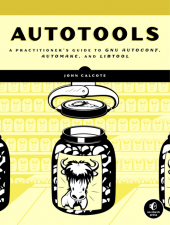
\includegraphics[width=0.6\textwidth]{slides/autotools-references/autotools-book.png}
  \end{columns}
\end{frame}

\begin{frame}{Official documentation}
  \begin{columns}
    \column{0.6\textwidth}
    \begin{itemize}
    \item The official reference documentation from GNU is also very
      good, once you have a good understanding of the basics.
    \item Autoconf\\
      {\small \url{http://www.gnu.org/software/autoconf/manual/}}
    \item Automake\\
      {\small \url{http://www.gnu.org/software/automake/manual/}}
    \item Libtool\\
      {\small \url{http://www.gnu.org/software/libtool/manual/}}
    \end{itemize}
    \column{0.4\textwidth}
    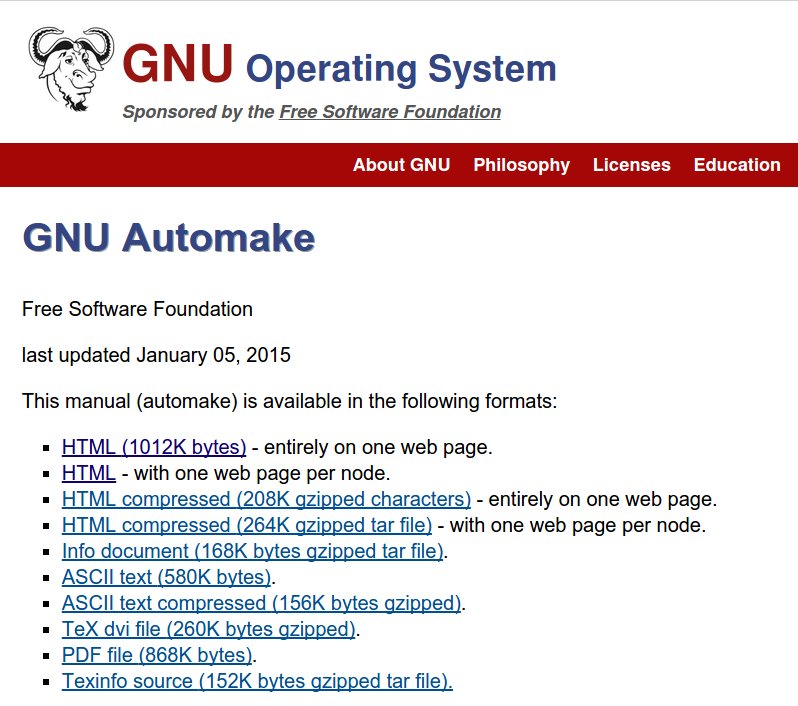
\includegraphics[width=\textwidth]{slides/autotools-references/automake-manual.png}
  \end{columns}
\end{frame}

\begin{frame}{Tutorials}
  \begin{columns}
    \column{0.6\textwidth}
    \begin{itemize}
    \item {\bf Autotools tutorial}, Alexandre Duret-Lutz,
      \url{https://www.lrde.epita.fr/~adl/autotools.html}
    \item {\bf Autotools Mythbuster}, Diego Elio “Flameeyes” Pettenò,
      \url{https://autotools.io/}
    \item {\bf Introduction to the Autotools}, David Wheeler, including
      a video, \url{http://www.dwheeler.com/autotools/}
    \end{itemize}
    \column{0.4\textwidth}
    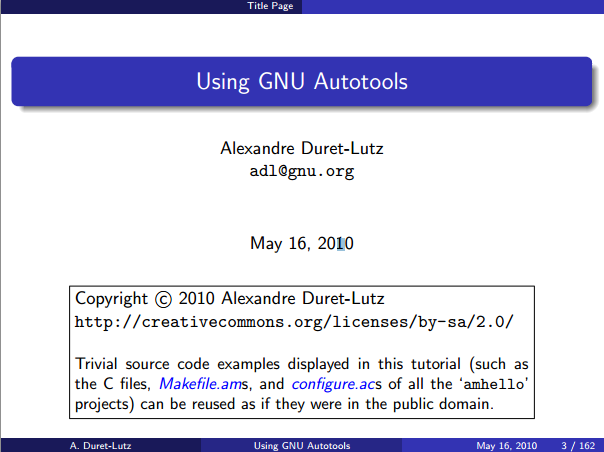
\includegraphics[width=\textwidth]{slides/autotools-references/autotools-tutorial.png}
  \end{columns}
\end{frame}

\begin{frame}{Use up to date materials}
  \begin{itemize}
  \item Be careful to use up-to-date material
    \begin{itemize}
    \item For example, the well-known book {\em GNU Autoconf, Automake
        and Libtool”} by Gary Vaughan et al., published originally in
      2000 is completely out of date
    \item Even though {\em autotools} are old, they have evolved quite
      significantly in recent times!
    \end{itemize}
  \end{itemize}
\end{frame}
